\documentclass[pdf]{beamer}
\mode<presentation>{} 
%% preamble
\usepackage{slidepacks}
\usepackage{hyperref}
\setbeamertemplate{caption}[numbered]
\usepackage[justification=centering]{caption}

\newcommand{\Lap}{\mathcal{L}}

\usetheme{Ilmenau}

\definecolor{camred}{RGB}{140, 21, 21} % camred (primary)
\definecolor{camlg}{RGB}{236, 236, 236}
\definecolor{camdg}{RGB}{217, 217, 217}
\setbeamercolor{palette primary}{bg=camred,fg=white}
\setbeamercolor{palette secondary}{bg=camdg,fg=black}
\setbeamercolor{palette tertiary}{bg=camlg,fg=black}
\setbeamercolor{palette quaternary}{bg=camlg,fg=black}
\setbeamercolor{structure}{fg=camred} % itemize, enumerate, etc
\setbeamercolor{section in toc}{fg=camred} % TOC sections

\definecolor{evandp}{RGB}{120, 66, 119}
\definecolor{evanlp}{RGB}{251, 241, 251}

\setbeamercolor{block title}{use=structure,fg=white,bg=evandp}
\setbeamercolor{block body}{use=structure,fg=black,bg=evanlp}

\beamertemplatenavigationsymbolsempty

\title[Randoms Correction]{New Randoms Correction Techniques \\ on the Gen II System}
\author[Eegan Ram]{Eegan Ram \texorpdfstring{\\}{}
\texorpdfstring{Stanford University}{}}
\date{\today}

\begin{document}


\begin{frame}
\thispagestyle{empty}          % prevents page numbering on the title slide
\titlepage
\end{frame}
\addtocounter{framenumber}{-1} % don't count title slide in the page numbering

\section{Introduction}

\begin{frame}{Randoms Correction}
    \begin{itemize}
        \item How many of the coincidences measured on a certain LOR are `random coincidences?'
        \item We use this information to advise image reconstruction.
    \end{itemize}
\end{frame}

\begin{frame}{Methods}
    \begin{itemize}
        \item Delayed-Window (DW)
        \item Singles-Rate (SR)
        \item Singles-Prompts (SP) - 2016, new to our group
        \item Singles-Prompts with Multiple Coincidence Correction - new
    \end{itemize}
\end{frame}

\begin{frame}{Delayed-Window (DW)}
    \begin{figure}[H]
        \centering
        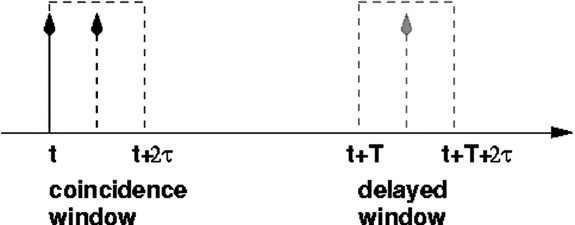
\includegraphics[width=0.8\textwidth]{figures/dwdemo.png}
    \end{figure}
    \begin{itemize}
        \item Every time you open a prompt window, also open a delayed window.
        \item A count in the DW $=$ random coincidence on that LOR.
        \item Currently implemented on hardware.
    \end{itemize}
\end{frame}

\begin{frame}{Singles-Rate (SR)}
    $$R_{ij} = 2 \rn{tau}{\tau} \rn{si}{S_i} \rn{sj}{S_j}$$
    \customanno{tau.north}{3em}{50}{coincidence window}{rotate=5}
    \customanno{si.south west}{3em}{-160}{\# singles in det $i$}{xshift=-7em, yshift=-0.7em}
    \customanno{sj.south east}{3em}{-40}{\# singles in det $j$}{}

    \vspace{2em}

    \begin{itemize}
        \item Estimates random coincidences from \# singles counts. 
        \item Requires singles acquisition.
    \end{itemize}
\end{frame}

\begin{frame}{Singles-Prompts (SR)}
    $$R_{ij}^{SP} = \frac{2 \tau e^{-(\lambda + S) \tau}}{(1 - 2 \lambda \tau)^2 }$$
\end{frame}

\section{Model}

\begin{frame}{Radius, Area, and Volume Equations}
    $$r(h) = \begin{cases}
    1.1 & 0 \leq h < 2 \\
    5.9164-6.02984h+2.52828h^2-0.418985h^3 + \\ 0.03203h^4 -0.000943h^5 & 2 < h < 9.5 \\
    5.5 & h \geq 9.5
\end{cases}$$
    The area and volume equations could then be easily derived via integral.
\end{frame}

\begin{frame}{Height and Exhaust Speed Equation}
    \begin{itemize}
        \item Used Newton's method to solve for $h(V(m))$.
        \item Then we could solve for $u$
    \end{itemize}


    $$u = -\rho \sqrt{\frac{2(\rho g h - P_{atm} + P_0 (1 + \frac{m_0 - \rho V(h)}{V_0 \rho})^{-\gamma}}{\rho (1 - (\frac{A_n}{A_h})^2)}}$$
\end{frame}

\section{Conclusion}

\begin{frame}{Conclusion}
    \begin{itemize}
        \item The rocket model did seem to match experiment quite well for masses and pressures in the middle range, but did seem to break down when the water level was too low or too high, as well as when the pressure was really low.
        \item One clear weakness of the experiment was that we didn't account for the rocket's horizontal motion and how that might have caused error. We felt like the math was too complicated given that the $Bv^2$ drag term made decomposing the velocity tedious.
        \item The horizontal angles made it really hard to tell what was experimental error and what wasn't.
    \end{itemize}
\end{frame}

\begin{frame}{Future Work}
    \begin{itemize}
        \item Work on a mathematical model to properly deal with diagonal launches.
        \item Work on a model to better correct for large angle discrepancies with the camera recording.
        \item More trials.
        \item Better fins for stability so drag measurements more useful.
    \end{itemize}
\end{frame}


\section{Acknowledgements}

\begin{frame}{Acknowledgements}
\begin{itemize}
\item Professor Devin 
\item Berni for figuring out that we mixed up $r$ and $d$
\item Everyone who carried water to the launch site
\item Everyone who we borrowed materials from
\end{itemize}
\end{frame}

\end{document}